\documentclass[../main/main.tex]{subfiles}

\newdate{date}{18}{12}{2019}


\begin{document}

\chapter{Widom's scaling theory. Block-spin Kadanoff's transformation}

\marginpar{ \textbf{Lecture 19.} \\  \displaydate{date}. \\ Compiled:  \today.}

\section{Static scaling hypothesis (Widom)}
It is used whenever you have a collective behaviour.
As \( T \rightarrow T_c^{\pm} \) we know that \( \xi \rightarrow L \). In this limit all the microscopic and intermediate scales are irrelevant. The length scale of the problem are \( a,L,\xi  \), but  \( \xi  \) is the only relevant length scale in the problem.

One should expect that, for \( t \sim 0 \), the free energy (better, its critical term) is invariant in form by a change of scale. This hypothesis is also suggested by experimental data such as the ones shown by Guggenheim for the gas phase diagrams and the ones shown for ferromagnetic materials at different temperatures.

Which are the experimental data which gives us this ideas? What you can see from experiment (Figure \ref{fig:19_1}) is that data from different temperatures, if scaled properly, collapse into two (one for \( t<0 \) and one for \( t>0 \)) unique curves.


\begin{figure}[h!]
\centering
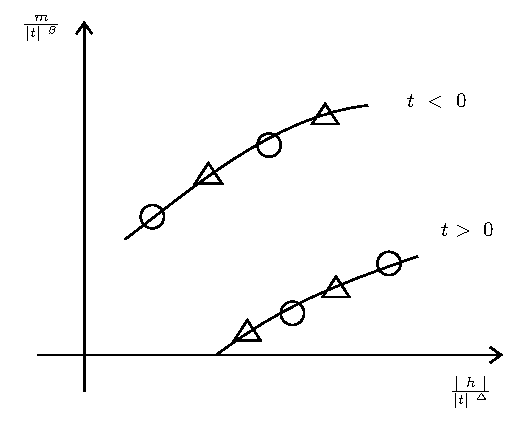
\includegraphics[width=0.5\textwidth]{../lessons/19_image/1.pdf}
\caption{\label{fig:19_1} Description.}
\end{figure}

The Widom's static scaling theory is introduced also to explain the collapse of data shown above.

In order to properly define the scaling hypothesis, we should rely on the mathematical concept of homogeneous functions.

\subsection{Homogeneous functions}
Consider a single variable \( r \).
\begin{definition}[Homogeneous function] \
\( f(r) \) is homogeneous in \( r \) if \( \forall \lambda \in \R \),
\begin{equation}
  f (\lambda r) = g (\lambda ) f(r)
\end{equation}
where \( g(\lambda ) \) is, for the moment, arbitrary.
\end{definition}
\begin{example}
  Parabola:
\begin{equation}
  f(r) = B r^2
\end{equation}
\begin{equation}
  f ( \lambda r) = B ( \lambda r)^2 = \lambda ^2 f (r) \quad \Rightarrow g ( \lambda ) = \lambda ^2
\end{equation}
\end{example}
\begin{remark}
An interesting property of an homogeneous function is that, if \( f(r_0) \) is known and \( g(\lambda ) \) is known, hence \( f(r) \) is known \( \forall r \in \R \).
Indeed, we can always write \( r=\lambda r_0 \),
\begin{equation}
  f(r) = f (\lambda r_0) = g(\lambda ) f(r_0)
\end{equation}
\end{remark}
\begin{theorem}[]
  The function \( g(\lambda ) \) is not arbitrary but it must be of the form
\begin{equation}
  g(\lambda ) = \lambda ^p
\end{equation}
where \( p \) is the degree of the homogeneity of the function.
\end{theorem}
\begin{proof}
Change of scale with respect to \( \mu  \) and \( \lambda  \).
\begin{equation}
  f(\lambda (\mu r)) = g (\lambda ) f(\mu r) = g(\lambda ) g(\mu ) f(r)
\end{equation}
On the other hand,
\begin{equation}
  f[(\lambda \mu )r] = g (\lambda  \mu ) f(r)
\end{equation}
Hence,
\begin{equation}
  g (\lambda \mu ) = g(\lambda ) g (\mu )
\end{equation}
Let us assume that \( g(\lambda ) \) is differentiable (actually \( g(\lambda ) \) continuous is sufficient but proof more complicated)
\begin{equation}
  \pdv{}{\mu } \qty[g(\lambda \mu )] = \pdv{}{\mu } \qty[ g(\lambda )g(\lambda )]
\end{equation}
\begin{equation}
  \Rightarrow \lambda g' (\lambda \mu ) = g (\lambda ) g' (\mu )
  \label{eq:19_1}
\end{equation}
Let \( \mu =1 \) and let \( g'(\mu =1) = p \), equation \eqref{eq:19_1} implies
\begin{equation}
  \frac{g'(\lambda )}{g(\lambda )} = \frac{p}{\lambda }
\end{equation}
\begin{equation}
  \dv{}{\lambda } \qty(\ln{g(\lambda )} ) = \frac{p}{\lambda }   \quad \Rightarrow \ln{g(\lambda )} = p \ln{\lambda } + c
\end{equation}
or
\begin{equation}
  g (\lambda ) = e^c \lambda ^p \quad \Rightarrow g'(\lambda ) = p e^c \lambda ^{p-1}
\end{equation}
and since \( g'(1) = p \), we have \( p=p e^c \) if and only if \( c=0 \) which implies
\begin{equation}
  g(\lambda ) = \lambda ^ p
\end{equation}
\end{proof}

\section{Generalized homogeneous functions}
We can make it for any variable, not only for a single one.
We are discussing \( f(x,y) \), that is a generalized homogeneous function if as a most general form as
\begin{equation}
  f (\lambda ^a x, \lambda ^b y) = \lambda f(x,y)
  \label{eq:19_2}
\end{equation}
Indeed, if we consider instead
\begin{equation}
    f (\lambda ^a x, \lambda ^b y) = \lambda^p f(x,y)
\end{equation}
we can always choose \( \lambda ^p \equiv s \) such that
\begin{equation}
  f ( s^{a/p} x, s^{b/p} y) = s f(x,y)
\end{equation}
and choosing \( a'=a/p \) and \( b'=b/p \) we are back to \eqref{eq:19_2}.
\begin{remark}
Since \( \lambda  \) is arbitrary \( \Rightarrow \lambda  = y ^{-1/b} \), we get
\begin{equation}
  f(x,y) = y^{1/b} f \qty( \frac{x}{y^{a/b}},1)
\end{equation}
\( f \) depends on \( x \) and \( y \) only through the ratio \( \frac{x}{y^{a/b}} \)! Similarly, for \( x \), one can choose \( \lambda = x^{-1/a} \).
\end{remark}
\begin{example}
Examples of non-homogeneous functions are
\begin{equation}
  f(x) = e^{-x}
\end{equation}
\begin{equation}
  f(x) = \log{x}
\end{equation}
\end{example}

\section{Widom's theory of static scaling}
Close to the critical point, the singular part of the free energy does not change form by a change of the scale.

More precisely, given \( t \equiv  \frac{T - T_c}{T_c}\) and \( h = \frac{H - H_c}{H_c} \) and the free energy density
\begin{equation}
  f (T,H) = f_{ana} (T,H) + f_{sing} (t,h)
\end{equation}
where \( f_{ana} \) is an analytic term and \( f_{sing} \) diverges, has a singularity. Given that the scaling hypothesis is
\begin{equation}
  f_s ( \lambda ^{p_1} t, \lambda ^{p_2} h) = \lambda f_s (t,h), \quad \forall \lambda \in \R
\end{equation}
where \( p_1 \) and \( p_2 \) are the degrees of the homogeneity of the singular part of the free energy.
\begin{remark}
The exponents \( p_1 \) and \( p_2 \)  are not specified by the hypothesis but they will depend on the critical exponents.
\end{remark}
\begin{remark}
Since \( f_s \) is a generalized homogeneous function, it is always possible to choose \( \lambda  \) to eliminate one dependence.

For example, one can choose \(   \lambda = h^{-1/p_2} \) to obtain
\begin{equation}
 f_s (t,h) = h^{1/p_2} f_s (h^{-p_1/p_2} t , 1)
\end{equation}
where
\begin{equation}
  \Delta  \equiv \frac{p_1}{p_2}
\end{equation}
is called the \emph{gap exponent}.
\end{remark}

Now, let us see how this simple hypothesis allow us, by simple differential calculus, to obtain relations between the thermodynamic critical exponents.

\subsection{Scaling of the magnetization}
Let us start from the scaling hypothesis
\begin{equation}
  f_s (\lambda ^{p_1}t, \lambda ^{p_2}h) = \lambda f_s (t,h)
  \label{eq:19_3}
\end{equation}
Since \( M \) is the \( 1^{st} \) derivative of \( f \) with respect to \( H \), let us derive   \eqref{eq:19_3} with respect to \( h \)
\begin{equation}
  \lambda ^{p_2} \pdv{f_s}{h} \qty(\lambda ^{p_1}t, \lambda ^{p_2}h) = \lambda \pdv{f_s}{h} (t,h)
\end{equation}
\begin{equation}
  \Rightarrow \lambda ^{p_2} M_s ( \lambda ^{p_1} t, \lambda ^{p_2} h) = \lambda M_s (t,h)
  \label{eq:19_4}
\end{equation}
On the other hand, we know that, for \( h=0 \) and \( t \rightarrow 0^- \), \( M_s (t) \sim (-t)^{\beta } \). Putting \( h=0 \) in \eqref{eq:19_4}
\begin{equation}
  M_s (t,0) = \lambda ^{p_2 -1} M_s ( \lambda ^{p_1} t,0)
\end{equation}
Since \( \lambda  \) is arbitrary, we can eliminate the dependence on \( t \) by choosing
\begin{equation}
  \lambda ^{p_1} t = -1 \quad \Rightarrow \lambda = (t)^{-1/p_1}
\end{equation}
hence,
\begin{equation}
  M_s (t,0) = - (t)^{\frac{1-p_2}{p_1}} M_s (-1,0)
\end{equation}
Obtaining the \( 1^{st} \) relation:
\begin{equation}
  \beta = \frac{1-p_2}{p_1}
\end{equation}
\subsubsection{Exponent \( \delta  \)}
At \( T=T_c \) \( (t=0) \) we have
\begin{equation}
   M_s  \overset{h \rightarrow 0^+}{\sim} h^{1/\delta }
\end{equation}
\begin{equation}
  \Rightarrow M_s (0,h) = \lambda ^{p_2 - 1} M_s (0,\lambda ^{p_2} h)
\end{equation}
Now, we want
\begin{equation}
  \lambda ^{p_1} h = 1 \quad \Rightarrow \lambda = h ^{-1/p_2}
\end{equation}
\begin{equation}
  \Rightarrow M_s (0,h) = h ^{\frac{1-p_2}{p_2}} M_s (0,1)
\end{equation}
Since \( M_s \sim h^{1/\delta } \), we get the \( 2^{nd} \) relation:
\begin{equation}
  \delta = \frac{p_2}{ 1 - p_2 }
\end{equation}
By getting \( p_1 \) and \( p_2 \) from the two relations we have
\begin{equation}
  p_1 = \frac{1}{\beta (\delta +1)}, \quad p_2 = \frac{\delta }{\delta + 1}
\end{equation}
and in particular the gap exponent is
\begin{equation}
  \frac{p_2}{p_1} \equiv  \Delta = \beta \delta
\end{equation}

\subsection{Equation of state}
We can also predict the scaling form of the equation of state and explain the collapse of the experimental data. Let us start from
\begin{equation}
  M_s (t,h) = \lambda ^{p_2 - 1} M_s (\lambda ^{p_1} t, \lambda ^{p_2} h)
\end{equation}
and choose \( \lambda = \abs{t}^{-1/p_1}  \).

We have
\begin{equation}
  M_s (t,h) = \abs{t}^{\frac{1-p_2}{p_1}} M_s ( \frac{t}{\abs{t} }, \frac{h}{\abs{t}^{\Delta } })
\end{equation}
Since \( \beta = \frac{1-p_2}{p_1} \), \( \delta = \frac{p_2}{p_1} \) we have
\begin{equation}
  \frac{M_s (t,h)}{\abs{t}^{\beta } } = M_s ( \frac{t}{\abs{t} }, \frac{h}{\abs{t}^{\Delta } })
  \label{eq:19_5}
\end{equation}
We define the \emph{scaled magnetization} as
\begin{equation}
  \bar{m} \equiv \abs{t}^{-\beta } M(t,h)
\end{equation}
and the \emph{scaled magnetic field} as
\begin{equation}
  \bar{h} \equiv \abs{t}^{-\Delta } h (t,M)
\end{equation}
Hence, the equation \eqref{eq:19_5} becomes
\begin{equation}
  \bar{m} = F_{\pm} (\bar{h} )
\end{equation}
universal curves!

\subsection{Magnetic susceptibility}
Compute \( \pdv[2]{}{h}  \) of the scaling hypothesis
\begin{equation}
  f_s ( \lambda^{p_1} t, \lambda ^{p_2}h) = \lambda f_s (t,h)
\end{equation}
From equation \eqref{eq:19_5} we have
\begin{equation}
  \lambda ^{2p_2} \chi _T \qty(\lambda ^{p_1}t, \lambda ^{p_2}h) = \lambda \chi _T (t,h)
\end{equation}
\subsubsection{Exponent \( \gamma   \) }
Consider \( h=0 \), \( t \rightarrow 0^- \) (for example).
 Let \( \lambda = - t ^{-1/p_1} \), from equation \eqref{eq:19_5}
\begin{equation}
  \chi _T (t,0) = \qty(-t)^{-\frac{2p_2-1}{p_1}} \chi _T (-1,0)
\end{equation}
and since
\begin{equation}
  \chi _T (t,0) \overset{t \rightarrow 0^-}{\sim } \qty(-t)^{-\gamma_-  }
\end{equation}
we get
\begin{equation}
  \gamma _- = \frac{2p_2 -1}{p_1} = \beta (\delta -1)
\end{equation}
\begin{remark}
For \( t \rightarrow 0^+ \), we have \( \lambda  = t ^{1/p_1} \) and we get
\begin{equation}
  \gamma _- = \gamma _+ \equiv \gamma  = \beta (\delta -1)
\end{equation}
relation between exponents!
\end{remark}

\subsection{Scaling of the specific heat}
Starting again from
\begin{equation}
  f_s ( \lambda^{p_1} t, \lambda ^{p_2}h) = \lambda f_s (t,h)
\end{equation}
and compute \( \pdv[2]{}{t}  \) of both side, we get
\begin{equation}
  \lambda ^{2p_1}c_h \qty(\lambda ^{p_1}t, \lambda ^{p_2}h) = \lambda c_H (t,h)
\end{equation}
For \( h=0 \) and \( t \rightarrow 0^- \), we have \( \lambda = (-t)^{-1/p_1} \) which implies
\begin{equation}
  - t^{-2} c_H (-1,0) = - t ^{-1/p_1} c_H (t,0)
\end{equation}
and since
\begin{equation}
  c_H (t,0) \overset{t \rightarrow 0^-}{\sim } t^{-\alpha _-}
\end{equation}
we get
\begin{equation}
  \alpha _- = 2 - \frac{1}{p_1}
  \label{eq:19_6}
\end{equation}
Also in this case it is easy to show that
\begin{equation}
  \alpha _- = \alpha _+
\end{equation}
Moreover, by inserting in \eqref{eq:19_6} the relation \( p_1 = \frac{1}{\beta (\delta +1)} \) one gets the \emph{Griffith relation}
\begin{equation}
  \alpha + \beta (\delta +1) = 2
\end{equation}
Moreover, by combining Griffith with the relation \( \gamma = \beta (\delta -1)  \) one get the \emph{Rushbrooke relation}
\begin{equation}
  \alpha + 2 \beta + \gamma = 2
\end{equation}
\begin{remark}
By using these hypothesis you can get equalities. All the inequality that you have in thermodynamics becames equalities. (lesson)
\end{remark}

\subsection{Second form of the static scaling hypothesis}
\begin{equation}
  f_s ( \lambda^{p_1} t, \lambda ^{p_2}h) = \lambda f_s (t,h)
\end{equation}
The relation \( \lambda = t ^{-1/p_1} \) implies
\begin{equation}
  f_s (1,t^{-p_2/p_1}h) = t^{-1/p_1} f_s (t,h)
\end{equation}
Since \( \Delta = \frac{p_2}{p_1} \) and \( \alpha = 2 - \frac{1}{p_1} \), one gets
\begin{equation}
  f_s (t,h) = t^{2- \alpha } f_s (1, \frac{h}{t^{\Delta }})
\end{equation}
that is the \( 2^{nd} \) scaling form of the free-energy.

\section{Kadanoff's block spin and scaling of the correlation function}
Widom's theory refers only to the free energy of the system. Moreover it do, not fully explain how the scaling hypothesis derives by \( \xi  \) being the only relevant length of the system.

The first argument on this point was given \( 1966 \) by Kadonoff.
The Kadonoff's intuition was: the divergence of \( \xi  \) implies a relation between the coupling constants of a \( \mathcal{H}_{eff} \) and the length scales over which \( m \) is defined.  


\section{lesson}

\section{Kadanoff 1966}
How can we relate the coupling costant of the two hamiltonian. This is the idea of the renormalization group.
\begin{equation}
  - \beta \mathcal{H}_{\Omega } = k \sum_{\expval{ij} }^{} \sigma _i \sigma _j + h \sum_{i}^{} \sigma _i
\end{equation}
with
\begin{equation}
  \sigma _i = \pm 1, \quad k \equiv \frac{J}{k_B T}, \quad h \equiv \frac{H}{k_B T}
\end{equation}
we assume
\begin{equation}
  r \ll \xi  \quad \Rightarrow a \ll l a \ll \xi (t)
\end{equation}
We can build up many procedure.
This is the \emph{Block spin transformation}, the idea is divide into cell of length \( la \) (figure 2) and we replace it with (figure 3).

\begin{equation}
  S_I \equiv \frac{1}{\abs{m_l} } \frac{1}{l^D} \sum_{i \in I}^{}  \sigma _i
\end{equation}
with the sum is over all the sites with a given cell.
Define the magnetization
\begin{equation}
  m_l \equiv \frac{1}{l^D} \sum_{i \in I}^{} \sigma _i
\end{equation}

The frist assumption is that the Hamiltonian of the new system \( \mathcal{H}_l \) is equal in form to \( \mathcal{H}_ \Omega  \). It means that we can write
\begin{equation}
  - \beta \mathcal{H}_l = k_l \sum_{\expval{IJ} }^{} S_I S_J  + h_l \sum_{I}^{} S_I
\end{equation}

\begin{equation}
  N_l = \frac{N}{l^D}
\end{equation}
How you measure in the new system the lengths? the correlations lengths. Before we have changed the size of the system. We have increased the ruler, so the number is smaller now. It seems stupid but it is fundamental.
\begin{equation}
  \xi _l = \frac{\xi }{l}
\end{equation}
were the last relation it is very important!

Anyway for the Kadanoff it does not meant so much because we do not iterate.
The new distance of the critical point in the new system \( t_l \) is
\begin{equation}
  t_l > t
\end{equation}

We have
\begin{equation}
  h \sum_{i}^{} \sigma _i = h \sum_{I}^{} \sum_{i \in \sigma _i}^{}  \sigma _i = h \sum_{I}^{}    \abs{m_l} l^D S_I
  = \underbrace{h \abs{m_l} l^D}_{h_l} \sum_{I}^{} S_I
\end{equation}
\begin{equation}
  h_l = \abs{m_l} l^D h
\end{equation}

What happens to the free energy?
Since \( h_l \) is equal in form to \( h \), the story is the same. So also for the free energy there would be a difference in the number of spins.

If I take \(   N_l f_s (t_l,h_l) \) this is equal to
\begin{equation}
  N_l f_s (t_l,h_l) = N f_s (t,h)
\end{equation}
\begin{equation}
  \Rightarrow  f_s (t_l,h_l) = l^D f_s (t,h)
\end{equation}

Somehow we are getting just for free \( \lambda \equiv l^D \). Now we need other assumptions. The second assumption is
\begin{equation}
  t_l = t l^{Y_t} \quad h_l = h l^{Y_h}
\end{equation}
\begin{equation}
  f_s (t,h) = l^{-D} f_s (t l^{Y_t}, h l^{Y_h})
\end{equation}
Let us take \( l= \abs{t}^{-1/Y_t}  \)
\begin{equation}
  f_s (t,h) = \abs{t}^{D/Y_t} f_s (1, h \abs{t}^{-Y_h/Y_t} )
\end{equation}
\begin{equation}
  \Delta = \frac{Y_h}{Y_t} \quad \Rightarrow 2 - \alpha = \frac{D}{Y_t}
\end{equation}
We are changing the ruler
\begin{equation}
  G_{IJ} (\va{r}_l, t_l) \equiv \expval{S_I S_J} - \expval{S_I}\expval{S_J}
\end{equation}
\begin{equation}
  \abs{\va{r}_l} = \frac{\va{r}}{l}
\end{equation}
We want to write \( G_{IJ} \) for \( \sigma _i \sigma _j \), what we get at the end is
\begin{equation}
  G_{IJ} (\va{r}_l, t_l) = l^{2(D-Y_h)} G_{ij} (\va{r},t)
\end{equation}

What we get resclaing the system is
\begin{equation}
  G_{IJ} \qty(\va{r}/l, t l ^{Y_t}, h l^{Y_h}) l^{2(D-Y_h)} G_{ij} (\va{r},t)
\end{equation}
\begin{equation}
  l = t^{-1/Y_t}
\end{equation}
\begin{equation}
  G_{IJ} (\va{r} t^{1/Y_t}, 1, h t^{-Y_h/Y_t}) = t^{-2 \frac{D- Y_h}{Y_t}} G_{ij} (\va{r},t)
\end{equation}





\end{document}
